\documentclass[a4paper]{article}
\usepackage{geometry}
\usepackage{graphicx}
\usepackage{natbib}
\usepackage{amsmath}
\usepackage{amssymb}
\usepackage{amsthm}
\usepackage{paralist}
\usepackage{epstopdf}
\usepackage{tabularx}
\usepackage{longtable}
\usepackage{multirow}
\usepackage{multicol}
\usepackage[hidelinks]{hyperref}
\usepackage{fancyvrb}
\usepackage{float}
\usepackage{paralist}
\usepackage[svgname]{xcolor}
\usepackage{enumerate}
\usepackage{array}
\usepackage{times}
\usepackage{url}
\usepackage{fancyhdr}
\usepackage{comment}
\usepackage{environ}
\usepackage{times}
\usepackage{textcomp}
\usepackage{caption}
\usepackage{bbm}
\usepackage{enumitem}
\usepackage{algorithm}
\usepackage{algpseudocode}
\usepackage{caption}
\usepackage{subcaption}
\usepackage{svg}


\urlstyle{rm}

\setlength\parindent{0pt} % Removes all indentation from paragraphs
\theoremstyle{definition}
\newtheorem{definition}{Definition}[]
\newtheorem{conjecture}{Conjecture}[]
\newtheorem{example}{Example}[]
\newtheorem{theorem}{Theorem}[]
\newtheorem{lemma}{Lemma}
\newtheorem{proposition}{Proposition}
\newtheorem{corollary}{Corollary}

\floatname{algorithm}{Procedure}
\renewcommand{\algorithmicrequire}{\textbf{Input:}}
\renewcommand{\algorithmicensure}{\textbf{Output:}}
\newcommand{\abs}[1]{\lvert#1\rvert}
\newcommand{\norm}[1]{\lVert#1\rVert}
\newcommand{\RR}{\mathbb{R}}
\newcommand{\CC}{\mathbb{C}}
\newcommand{\Nat}{\mathbb{N}}
\newcommand{\br}[1]{\{#1\}}
\DeclareMathOperator*{\argmin}{arg\,min}
\DeclareMathOperator*{\argmax}{arg\,max}
\renewcommand{\qedsymbol}{$\blacksquare$}

\definecolor{dkgreen}{rgb}{0,0.6,0}
\definecolor{gray}{rgb}{0.5,0.5,0.5}
\definecolor{mauve}{rgb}{0.58,0,0.82}

\newcommand{\Var}{\mathrm{Var}}
\newcommand{\Cov}{\mathrm{Cov}}

\newcommand{\vc}[1]{\boldsymbol{#1}}
\newcommand{\xv}{\vc{x}}
\newcommand{\Sigmav}{\vc{\Sigma}}
\newcommand{\alphav}{\vc{\alpha}}
\newcommand{\muv}{\vc{\mu}}

\newcommand{\red}[1]{\textcolor{red}{#1}}

\def\x{\mathbf x}
\def\y{\mathbf y}
\def\w{\mathbf w}
\def\v{\mathbf v}
\def\E{\mathbb E}
\def\V{\mathbb V}
\def\ind{\mathbbm 1}

% TO SHOW SOLUTIONS, include following (else comment out):
\newenvironment{soln}{
	\leavevmode\color{blue}\ignorespaces
}{}

\hypersetup{
	%    colorlinks,
	linkcolor={red!50!black},
	citecolor={blue!50!black},
	urlcolor={blue!80!black}
}

\geometry{
	top=1in,            % <-- you want to adjust this
	inner=1in,
	outer=1in,
	bottom=1in,
	headheight=3em,       % <-- and this
	headsep=2em,          % <-- and this
	footskip=3em,
}


\pagestyle{fancyplain}
\lhead{\fancyplain{}{Homework 6}}
\rhead{\fancyplain{}{CS 760 Machine Learning}}
\cfoot{\thepage}

\title{\textsc{Homework 6}} % Title

%%% NOTE:  Replace 'NAME HERE' etc., and delete any "\red{}" wrappers (so it won't show up as red)

\author{
	\red{APOORVA KUMAR} \\
	\red{908 461 5997}\\
} 

\date{}

\begin{document}
	
	\maketitle 
	
        \textbf{Instructions:}
        Use this latex file as a template to develop your homework. We are changing our reproducibility policy on code submissions going forward. \textbf{Instead of uploading it on GitHub, please submit a separate zip file that contains your code. You will submit two files to Canvas, one is your pdf, and the other one is a zip file.} Late submissions may not be accepted. You can choose any programming language (i.e. python, R, or MATLAB). Please check Piazza for updates about the homework.
        \vspace{0.1in}
	
	\section{Implementation: GAN (30 pts)}
	In this part, you are expected to implement GAN with MNIST dataset. We have provided a base jupyter notebook (gan-base.ipynb) for you to start with, which provides a model setup and training configurations to train GAN with MNIST dataset.
	
	\begin{enumerate} [label=(\alph*)]
		\item Implement training loop and report learning curves and generated images in epoch 1, 50, 100. Note that drawing learning curves and visualization of images are already implemented in provided jupyter notebook. \hfill (15 pts)
		
		\begin{algorithm}
			\caption{Training GAN, modified from \cite{goodfellow2014generative}}\label{alg:GAN}
			\begin{algorithmic}
				\Require $m$: real data batch size, $n_{z}$: fake data batch size
				\Ensure Discriminator $D$, Generator $G$
				
				\For{number of training iterations}
				
				\State{$\#$ Training discriminator}
				\State{Sample minibatch of $n_{z}$ noise samples $\{z^{(1)}, z^{(2)}, \cdots, z^{(n_{z})}\}$ from noise prior $p_{g}(z)$}
				\State{Sample minibatch of $\{x^{(1)}, x^{(2)}, \cdots, x^{(m)}\}$}
				\State{Update the discriminator by ascending its stochastic  gradient:
					$$\nabla_{\theta_{d}} \big ( \cfrac{1}{m}  \sum_{i=1}^{m}  \log D(x^{(i)})  + \cfrac{1}{n_{z}} \sum_{i=1}^{n_{z}}  \log (1-D(G(z^{(i)})))\big )$$
				}
				
				\State{$\#$ Training generator}
				\State{Sample minibatch of $n_{z}$ noise samples $\{z^{(1)}, z^{(2)}, \cdots, z^{(n_{z})}\}$ from noise prior $p_{g}(z)$}
				\State{Update the generator  by ascending its stochastic  gradient:
					$$\nabla_{\theta_{g}}  \cfrac{1}{n_{z}} \sum_{i=1}^{n_{z}}  \log D(G(z^{(i)}))\big )$$
				}
				\EndFor
				
				\State{$\#$ The gradient-based updates can use any standard gradient-based learning rule. In the base code, we are using Adam optimizer \citep{kingma2014adam}}
			\end{algorithmic}
		\end{algorithm}
		
		Expected results are as follows.
		
		\begin{figure}[H]
			\centering
			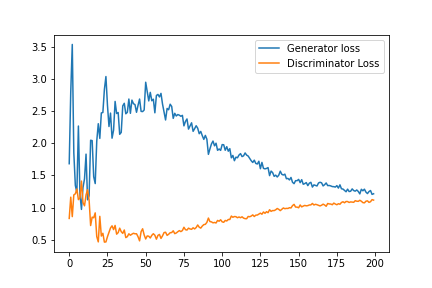
\includegraphics[width=0.7\textwidth]{Images/Base/gan_q1_loss.png}
			\caption{Learning curve}
			\label{fig:gan_q1_loss}
		\end{figure}
		
		\begin{figure}[H]
			\centering
			\begin{subfigure}[b]{0.3\textwidth}
				\centering
				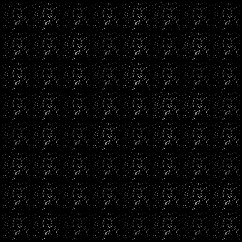
\includegraphics[width=\textwidth]{Images/Base/gan_q1_epoch1.png}
				\caption{epoch 1}
			\end{subfigure}
			\hfill
			\begin{subfigure}[b]{0.3\textwidth}
				\centering
				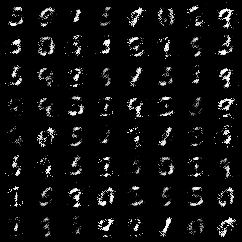
\includegraphics[width=\textwidth]{Images/Base/gan_q1_epoch50.png}
				\caption{epoch 50}
			\end{subfigure}
			\hfill
			\begin{subfigure}[b]{0.3\textwidth}
				\centering
				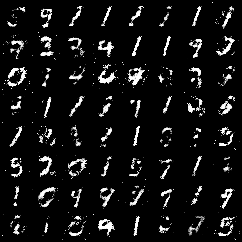
\includegraphics[width=\textwidth]{Images/Base/gan_q1_epoch100.png}
				\caption{epoch 100}
			\end{subfigure}
			\caption{Generated images by $G$}
			\label{fig:three graphs}
		\end{figure}
		
		
		\begin{soln}
                Solution begins here:
                \begin{figure}[H]
    			\centering
    			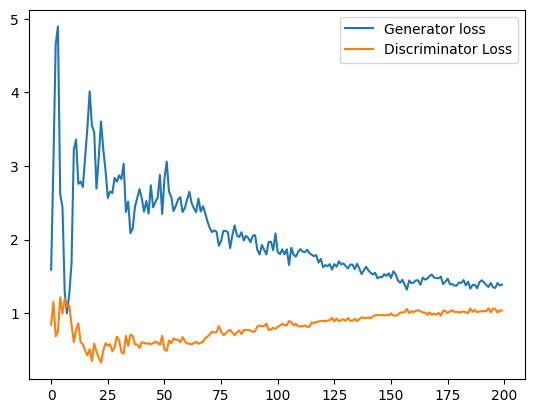
\includegraphics[width=0.6\textwidth]{Images/Q1/Q1a_train.png}
    			\caption{Solution Learning curve}
    			\label{fig:gan_q1a_loss}
    		\end{figure}
                \begin{figure}[H]
    			\centering
    			\begin{subfigure}[b]{0.3\textwidth}
    				\centering
    				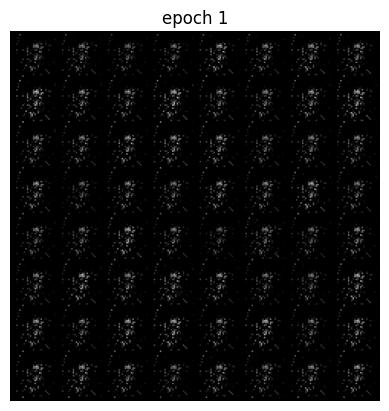
\includegraphics[width=\textwidth]{Images/Q1/Q1a_1.png}
    				\caption{Epoch 1}
    			\end{subfigure}
    			\hfill
    			\begin{subfigure}[b]{0.3\textwidth}
    				\centering
    				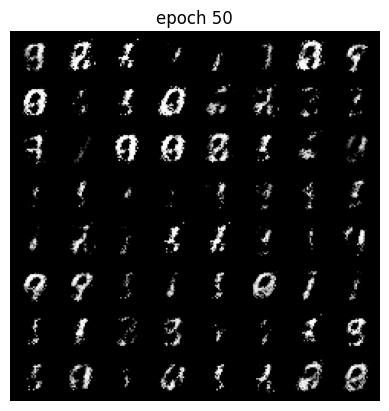
\includegraphics[width=\textwidth]{Images/Q1/Q1a_50.png}
    				\caption{Epoch 50}
    			\end{subfigure}
    			\hfill
    			\begin{subfigure}[b]{0.3\textwidth}
    				\centering
    				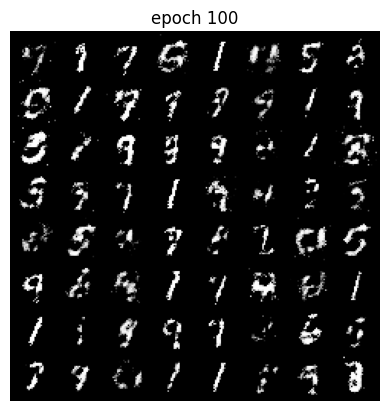
\includegraphics[width=\textwidth]{Images/Q1/Q1a_100.png}
    				\caption{Epoch 100}
    			\end{subfigure}
    			\caption{Solution Generated images by $G$}
    			\label{fig:sol1a graphs}
    		\end{figure} 
            \end{soln}
		
		
		
		\item Replace the generator update rule as the original one in the slide,\\
		``Update the generator by descending its stochastic gradient:
		
		$$\nabla_{\theta_{g}}  \cfrac{1}{n_{z}}  \sum_{i=1}^{n_{z}}\log (1-D(G(z^{(i)})))\big )$$
		"
		, and report learning curves and generated images in epoch 1, 50, 100. Compare the result with (a). Note that it may not work. If training does not work, explain why it doesn't work.
		\hfill (10 pts)
		
		\begin{soln}  
                Here we see that the training doesn't work because the gradients start to saturate early during the training causing the Discriminator to reject every sample out of the Generator because of how the loss function works. In part (a) we maximize $\log{D(G(z))}$ which provides us with enough opposite directional gradient during early training for the Generator to move in the right direction. On the other hand during the training of this part we see that loss function can be brought down easily just by the Discriminator thus providing no gradient to the Generator to learn anything. The same can also be seen on the learning curve which hits zero instantaneously. 
                \begin{figure}[H]
    			\centering
    			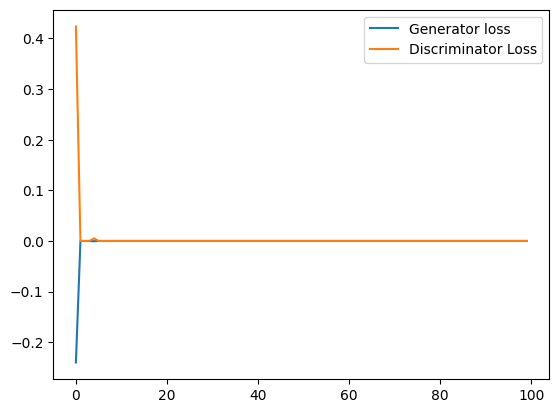
\includegraphics[width=0.6\textwidth]{Images/Q1/Q1b_train.png}
    			\caption{Solution Learning curve}
    			\label{fig:gan_q1b_loss}
    		\end{figure}
                \begin{figure}[H]
    			\centering
    			\begin{subfigure}[b]{0.3\textwidth}
    				\centering
    				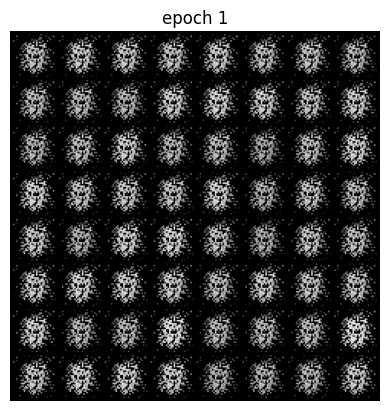
\includegraphics[width=\textwidth]{Images/Q1/Q1b_1.png}
    				\caption{Epoch 1}
    			\end{subfigure}
    			\hfill
    			\begin{subfigure}[b]{0.3\textwidth}
    				\centering
    				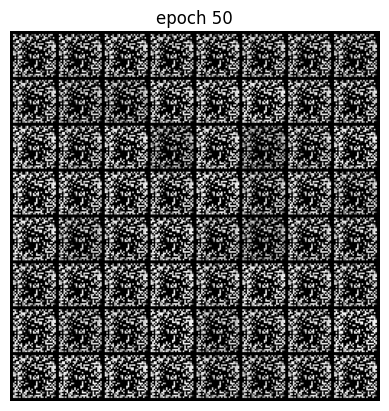
\includegraphics[width=\textwidth]{Images/Q1/Q1b_50.png}
    				\caption{Epoch 50}
    			\end{subfigure}
    			\hfill
    			\begin{subfigure}[b]{0.3\textwidth}
    				\centering
    				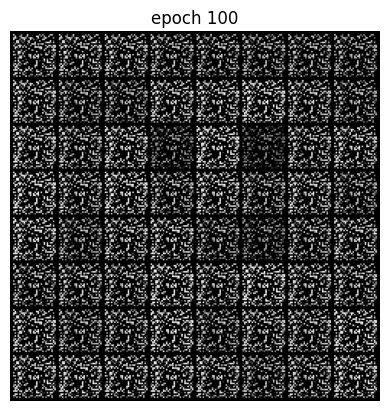
\includegraphics[width=\textwidth]{Images/Q1/Q1b_100.png}
    				\caption{Epoch 100}
    			\end{subfigure}
    			\caption{Solution Generated images by $G$}
    			\label{fig:sol1b graphs}
    		\end{figure}
            \end{soln}
		
		\item Except the method that we used in (a), how can we improve training for GAN? Implement that and report your setup, learning curves, and generated images in epoch 1, 50, 100.
		\hfill (5 pts)
		
		  \begin{soln}  
                We know that the main task of Generator is to fool the Discriminator into thinking its a true sample. Due to the way neural networks work its very easy to learn certain feature relation to classify and make decisions while neglecting other features in the set. The Generator can easily exploit this issue and build a model which achieves this relation without caring about the values of the other features. Thus our major task is to make the Discriminator more robust which inturn will make the Generator better. In an attempt to achieve this I set the true labels to 0.5 rather than 1 with a probability of 0.4 confusing the Discriminator. Its like an implicit dropout to force the Discriminator to learn better and make better connections. While this might result in a worse learning curve the output of the Generator can be seen to be much better than part (a).

                \begin{figure}[H]
    			\centering
    			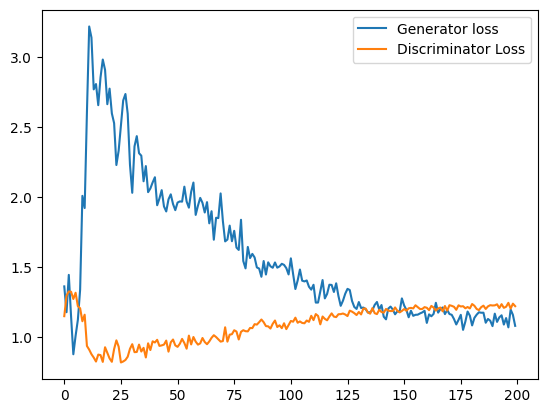
\includegraphics[width=0.6\textwidth]{Images/Q1/Q1c_train.png}
    			\caption{Solution Learning curve}
    			\label{fig:gan_q1c_loss}
    		\end{figure}
                \begin{figure}[H]
    			\centering
    			\begin{subfigure}[b]{0.3\textwidth}
    				\centering
    				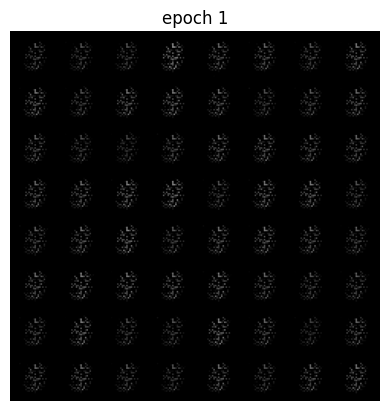
\includegraphics[width=\textwidth]{Images/Q1/Q1c_1.png}
    				\caption{Epoch 1}
    			\end{subfigure}
    			\hfill
    			\begin{subfigure}[b]{0.3\textwidth}
    				\centering
    				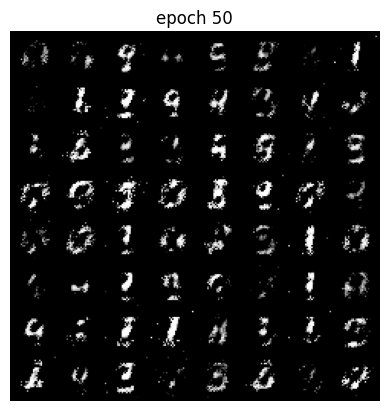
\includegraphics[width=\textwidth]{Images/Q1/Q1c_50.png}
    				\caption{Epoch 50}
    			\end{subfigure}
    			\hfill
    			\begin{subfigure}[b]{0.3\textwidth}
    				\centering
    				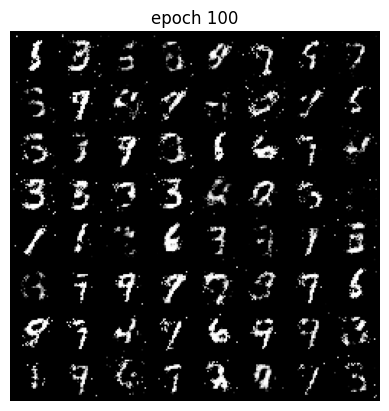
\includegraphics[width=\textwidth]{Images/Q1/Q1c_100.png}
    				\caption{Epoch 100}
    			\end{subfigure}
    			\caption{Solution Generated images by $G$}
    			\label{fig:sol1c graphs}
    		\end{figure}
  
            \end{soln}
		
	\end{enumerate}

	\section{Review change of variables in probability density functions [25 pts]} In Flow based generative model, we have seen $p_{\theta}(x)=p(f_{\theta}(x))|\frac{\partial f_{\theta}(x)}{\partial x}|$. As a hands-on (fixed parameter) example, consider the following setting.\\
	Let $X$ and $Y$ be independent, standard normal random variables. Consider the transformation $U=X+Y$ and $V=X-Y$. In the notation used above, $U=g_{1}(X, Y)$ where $g_{1}(X, Y)$ where $g_{1}(x, y)=x+y$ and $V=g_{2}(X, Y)$ where $g_{2}(x,y)=x-y$. The joint pdf of $X$ and $Y$ is $f_{X, Y}=(2\pi)^{-1} exp(-x^{2}/2) exp(-y^{2}/2), -\infty < x < \infty, -\infty < y < \infty$. Then, we can determine $u, v$ values by $x, y$, i.e. 
	$
	\begin{bmatrix}
		u\\
		v
	\end{bmatrix}
	$
	$=\begin{bmatrix}
		1 & 1 \\ 
		1 & -1
	\end{bmatrix}
	$
	$
	\begin{bmatrix}
		x\\
		y
	\end{bmatrix}
	$
	.
	
	\begin{enumerate}[label=(\alph*)]
		\item Compute Jacobian matrix $$J=\begin{bmatrix}
			\cfrac{\partial x}{\partial u} & \cfrac{\partial x}{\partial v}\\
			\cfrac{\partial y}{\partial u} & \cfrac{\partial y}{\partial v}
		\end{bmatrix}
		$$
		\hfill (5 pts)
		
		\begin{soln}
                $$x=\frac{1}{2}(u+v) \text{and} y=\frac{1}{2}(u-v)$$
                \begin{align*}
                    J =& \begin{bmatrix}
			                 \cfrac{\frac{1}{2}\partial (u+v)}{\partial u} & \cfrac{\frac{1}{2}\partial (u+v)}{\partial v}\\
			                 \cfrac{\frac{1}{2}\partial (u-v)}{\partial u} & \cfrac{\frac{1}{2}\partial (u-v)}{\partial v}
		              \end{bmatrix} \\
                    J =& \begin{bmatrix}
			                 \cfrac{1}{2} & \cfrac{1}{2}\\
			                 \cfrac{1}{2} & -\cfrac{1}{2}
		              \end{bmatrix}
                \end{align*}
            \end{soln}
		
		
		\item (Forward) Show that the joint pdf of U, V is
		$$f_{U, V}(u, v)=\big (\cfrac{1}{\sqrt{2\pi}\sqrt{2}}exp(-u^{2}/4)\big ) \big (\cfrac{1}{\sqrt{2\pi}\sqrt{2}}exp(-v^{2}/4)\big )$$
		\hfill (10 pts) \\
		(Hint: $f_{U, V}(u, v)=f_{X, Y}(?, ?)|det(J)|$) \\
		
		\begin{soln}
                $$\abs{det(J)} = \abs{-\cfrac{1}{2}\cfrac{1}{2}-\cfrac{1}{2}\cfrac{1}{2}} = \cfrac{1}{2}$$
                Thus we solve for $f_{U, V}(u, v)=\cfrac{1}{2}f_{X, Y}(\frac{1}{2}(u+v), \frac{1}{2}(u-v))$
                \begin{align*}
                    f_{U, V} &= \cfrac{1}{2}\frac{1}{2\pi} exp(-\frac{1}{4}(u+v)^{2}\frac{1}{2}) exp(-\frac{1}{4}(u-v)^{2}\frac{1}{2}) \\
                    &= \cfrac{1}{4\pi} exp(-\frac{1}{8}(u^2+v^2+2uv)) exp(-\frac{1}{8}(u^2+v^2-2uv)) \\
                    &= \cfrac{1}{4\pi} exp(-\frac{u^2}{4}) exp(-\frac{v^2}{4}) \\
                    \mathbf{f_{U, V}} &= \mathbf{\left(\cfrac{1}{\sqrt{2}\sqrt{2\pi}}exp\left(-\frac{u^2}{4}\right)\right) \left(\cfrac{1}{\sqrt{2}\sqrt{2\pi}}exp\left(-\frac{v^2}{4}\right)\right)}
                \end{align*}
            \end{soln}
		
		\item (Inverse) Check whether the following equation holds or not.
		$$f_{X, Y}(x, y)=f_{U, V}(x+y, x-y)|det(J)^{-1}|$$
		
		\hfill (10 pts) 
		  
		\begin{soln}
                $$\abs{det(J)^{-1}} = 2$$
                Thus we solve for $f_{X, Y}(x, y)=2f_{U, V}(x+y, x-y)$
                \begin{align*}
                    f_{X, Y} &= 2\left(\cfrac{1}{\sqrt{2}\sqrt{2\pi}}exp\left(-\frac{(x+y)^2}{4}\right)\right) \left(\cfrac{1}{\sqrt{2}\sqrt{2\pi}}exp\left(-\frac{(x-y)^2}{4}\right)\right) \\
                    &= 2\cfrac{1}{4\pi}exp\left(-\cfrac{(x+y)^2+(x-y)^2}{4}\right) \\
                    &= \cfrac{1}{2\pi}exp\left(-\cfrac{2x^2+2y^2}{4}\right) \\
                    &= \mathbf{\cfrac{1}{2\pi}exp\left(-\cfrac{x^2}{2}\right)exp\left(-\cfrac{y^2}{2}\right)}
                \end{align*}
                Hence we see that our original joint distribution was recovered.
            \end{soln}
	\end{enumerate}

\section{Directed Graphical Model [20 points]}
Consider the directed graphical model (aka Bayesian network) in Figure~\ref{fig:bn}.
\begin{figure}[H]
    \centering
    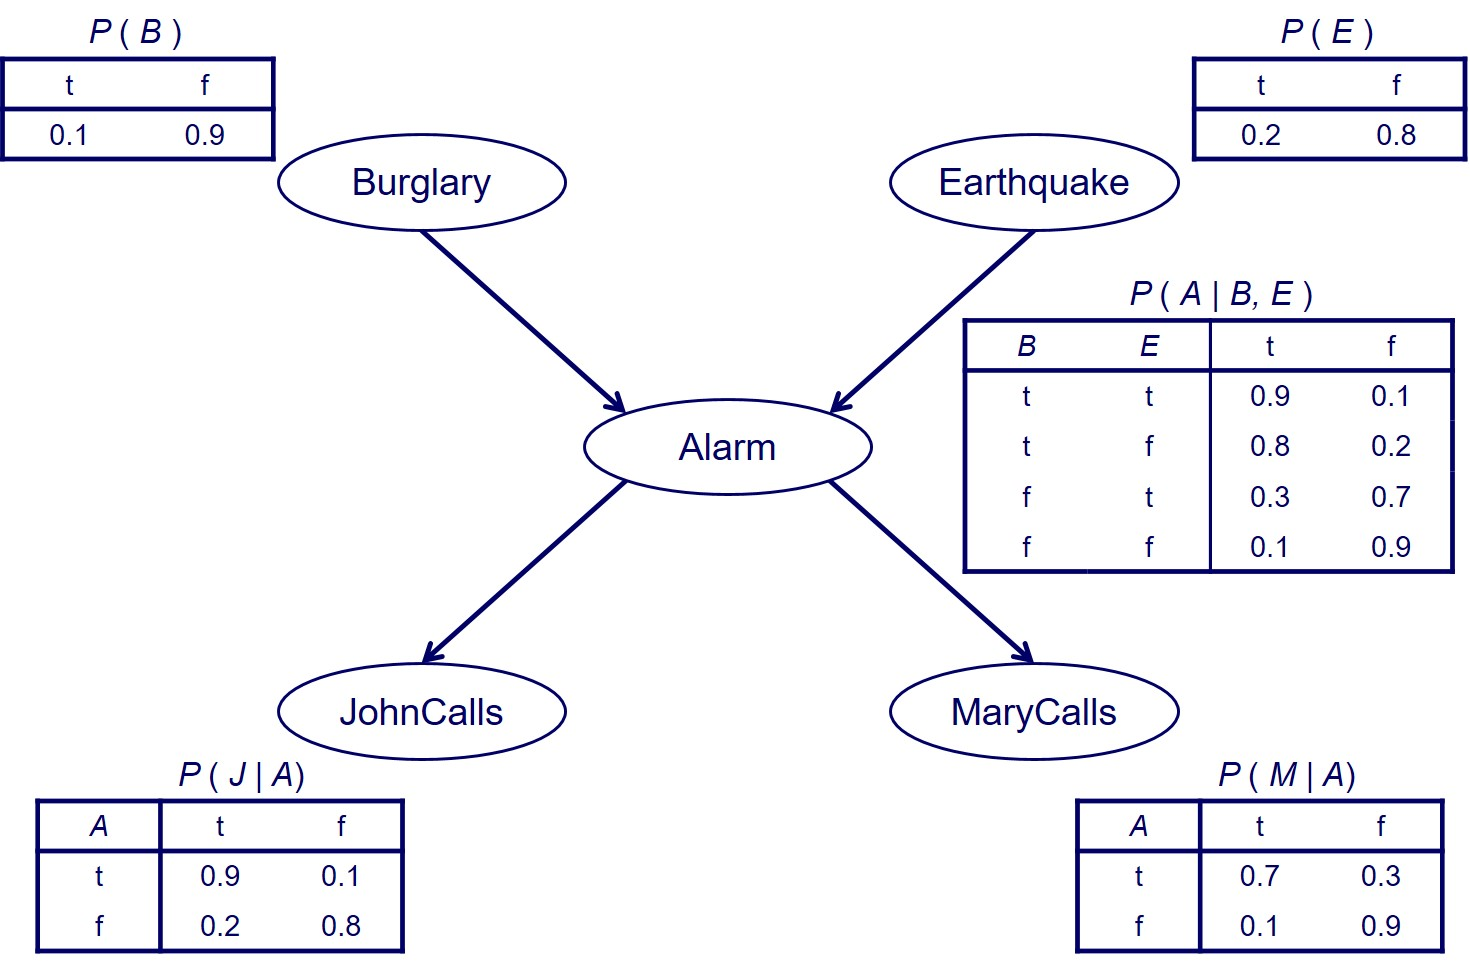
\includegraphics[width=0.8\textwidth]{Images/Base/BN.jpg}
    \caption{A Bayesian Network example.}
    \label{fig:bn}
\end{figure}
Compute $P(B=t \mid E=f,J=t,M=t)$ and $P(B=t \mid E=t,J=t,M=t)$. (10 points for each) These are the conditional probabilities of a burglar in your house (yikes!) when both of your neighbors John and Mary call you and say they hear an alarm in your house, but without or with an earthquake also going on in that area (what a busy day), respectively.

\begin{soln}
    Denote short hand notations as $B_f$ meaning $B=f$ or $E_t$ meaning $E=t$.
    Thus using Bayes Rule we can write:
    $$
        P(B_t \mid E_f, J_t, M_t) = \cfrac{P(B_t,E_f,J_t,M_t)}{P(B_t,E_f,J_t,M_t)+P(B_f,E_f,J_t,M_t)}
    $$
    Using condition probabilities we can write:
    \begin{multline*}
        P(B_t,E_f,J_t,M_t)=P(B_t)P(E_f)P(A_t\mid B_t,E_f)P(J_t\mid A_t)P(M_t\mid A_t) + \\ P(B_t)P(E_f)P(A_f\mid B_t,E_f)P(J_t\mid A_f)P(M_t\mid A_f)
    \end{multline*}
    $$P(B_t,E_f,J_t,M_t) = 0.1*0.8*0.8*0.9*0.7 + 0.1*0.8*0.2*0.2*0.1 = 0.04032 + 0.00032 = 0.04064$$
    \begin{multline*}
        P(B_f,E_f,J_t,M_t)=P(B_f)P(E_f)P(A_t\mid B_f,E_f)P(J_t\mid A_t)P(M_t\mid A_t) + \\ P(B_f)P(E_f)P(A_f\mid B_f,E_f)P(J_t\mid A_f)P(M_t\mid A_f)
    \end{multline*}
    $$P(B_f,E_f,J_t,M_t) = 0.9*0.8*0.1*0.9*0.7 + 0.9*0.8*0.9*0.2*0.1 =0.04536+0.01296= 0.05832$$
    \begin{align*}
        P(B_t \mid E_f, J_t, M_t) &= \cfrac{P(B_t,E_f,J_t,M_t)}{P(B_t,E_f,J_t,M_t)+P(B_f,E_f,J_t,M_t)} \\
        &= \cfrac{0.04064}{0.04064+0.05832} \\
        \mathbf{P(B=t \mid E=f, J=t, M=t)} &= \mathbf{0.41067}
    \end{align*}
    Similarily using the same for the second equation:
    $$
        P(B_t \mid E_t, J_t, M_t) = \cfrac{P(B_t,E_t,J_t,M_t)}{P(B_t,E_t,J_t,M_t)+P(B_f,E_t,J_t,M_t)}
    $$
    Using condition probabilities we can write:
    \begin{multline*}
        P(B_t,E_t,J_t,M_t)=P(B_t)P(E_t)P(A_t\mid B_t,E_t)P(J_t\mid A_t)P(M_t\mid A_t) + \\ P(B_t)P(E_t)P(A_f\mid B_t,E_t)P(J_t\mid A_f)P(M_t\mid A_f)
    \end{multline*}
    $$P(B_t,E_t,J_t,M_t) = 0.1*0.2*0.9*0.9*0.7 + 0.1*0.2*0.1*0.2*0.1 = 0.01134 + 0.00004 = 0.01138$$
    \begin{multline*}
        P(B_f,E_t,J_t,M_t)=P(B_f)P(E_t)P(A_t\mid B_f,E_t)P(J_t\mid A_t)P(M_t\mid A_t) + \\ P(B_f)P(E_t)P(A_f\mid B_f,E_t)P(J_t\mid A_f)P(M_t\mid A_f)
    \end{multline*}
    $$P(B_f,E_t,J_t,M_t) = 0.9*0.2*0.3*0.9*0.7 + 0.9*0.2*0.7*0.2*0.1 =0.03402+0.00252= 0.03654$$
    \begin{align*}
        P(B_t \mid E_t, J_t, M_t) &= \cfrac{P(B_t,E_t,J_t,M_t)}{P(B_t,E_t,J_t,M_t)+P(B_f,E_t,J_t,M_t)} \\
        &= \cfrac{0.01138}{0.01138+0.03654} \\
        \mathbf{P(B=t \mid E=t, J=t, M=t)} &= \mathbf{0.23748}
    \end{align*}
\end{soln}


\section{Chow-Liu Algorithm [25 pts]}
Suppose we wish to construct a directed graphical model for 3 features $X$, $Y$, and $Z$ using the Chow-Liu algorithm. We are given data from 100 independent experiments where each feature is binary and takes value $T$ or $F$. Below is a table summarizing the observations of the experiment:

\begin{table}[H]
        \centering
                \begin{tabular}{cccc}
                           $X$ & $Y$ & $Z$ & Count \\
                                \hline
                                T & T & T & 36 \\
                                \hline
                                T & T & F & 4 \\
                                \hline
                                T & F & T & 2 \\
                                \hline
                                T & F & F & 8 \\
                                \hline
                                F & T & T & 9 \\
                                \hline
                                F & T & F & 1 \\
                                \hline
                                F & F & T & 8 \\
                                \hline
                                F & F & F & 32 \\
                                \hline
                \end{tabular}
\end{table}
    \begin{soln}
        Lets first write the probabilities:
        \begin{itemize}
            \item $P_X(T)=0.5,P_X(F)=0.5$
            \item $P_Y(T)=0.5,P_Y(F)=0.5$
            \item $P_Z(T)=0.55,P_Z(F)=0.45$
            \item $P_{X,Y}(T,T)=0.4,P_{X,Y}(T,F)=0.1,P_{X,Y}(F,T)=0.1,P_{X,Y}(F,F)=0.4$
            \item $P_{Y,Z}(T,T)=0.45,P_{Y,Z}(T,F)=0.05,P_{Y,Z}(F,T)=0.1,P_{Y,Z}(F,F)=0.4$
            \item $P_{X,Z}(T,T)=0.38,P_{X,Z}(T,F)=0.12,P_{X,Z}(F,T)=0.17,P_{X,Z}(F,F)=0.33$
        \end{itemize}
    \end{soln}
\begin{enumerate}
	\item Compute the mutual information $I(X, Y)$ based on the frequencies observed in the data. (5 pts)
        \begin{soln}
            \begin{align*}
                I(X;Y) &= 0.4*\log_2(\frac{0.4}{0.5*0.5})+0.1*\log_2(\frac{0.1}{0.5*0.5})+0.1*\log_2(\frac{0.1}{0.5*0.5})+0.4*\log_2(\frac{0.4}{0.5*0.5}) \\
                &= 0.27122 - 0.1322 - 0.1322 + 0.27122 = \mathbf{0.27807}
            \end{align*}
        \end{soln}
	\item Compute the mutual information $I(X, Z)$ based on the frequencies observed in the data. (5 pts)
        \begin{soln}
            \begin{align*}
                I(X;Z) &= 0.38*\log_2(\frac{0.38}{0.5*0.55})+0.12*\log_2(\frac{0.12}{0.5*0.45})+0.1*\log_2(\frac{0.17}{0.5*0.55})+0.4*\log_2(\frac{0.33}{0.5*0.45}) \\
                &= 0.17729 - 0.10882 - 0.11796 + 0.18233 = \mathbf{0.13284}
            \end{align*}
        \end{soln}
	\item Compute the mutual information $I(Z, Y)$ based on the frequencies observed in the data. (5 pts)
        \begin{soln}
            \begin{align*}
                I(Z;Y) &= 0.45*\log_2(\frac{0.45}{0.5*0.55})+0.05*\log_2(\frac{0.05}{0.5*0.45})+0.1*\log_2(\frac{0.1}{0.5*0.55})+0.4*\log_2(\frac{0.4}{0.5*0.45}) \\
                &= 0.31972 - 0.10849 - 0.14594 + 0.33202  = \mathbf{0.39731}
            \end{align*}
        \end{soln}
	\item Which undirected edges will be selected by the Chow-Liu algorithm as the maximum spanning tree? (5 pts)
        \begin{soln}
            We arrange the Mutual Information in descending order as below:\\
            $I=\{I(Z,Y),I(X,Y),I(X,Z)\}$
            According to Chow Liu we first connect the nodes with highest Mutual Information, hence we first connect Y to Z and then Y to X and X to Z are connected already.
            
            \includesvg{Images/Q4_4}
        \end{soln}
	\item Root your tree at node $X$, assign directions to the selected edges. (5 pts)
        
        \begin{soln}
            \includesvg{Images/Q4_5}
        \end{soln}
\end{enumerate}

	\bibliography{hw6}
	\bibliographystyle{apalike}
\end{document}
